\documentclass[conference,12pt]{IEEEtran}
\usepackage{graphicx}
\usepackage{amsmath}
\usepackage{lipsum}
\usepackage{setspace}

% Set line spacing to match 12pt font size convention
\setstretch{1}

\begin{document}

\title{BIGDATA AND MACHINE LEARNING}
\author{Sakshi Patel }\\


\maketitle{\textbf{Assignment 1: Raw Data to Feature Space}}
\section{Task 1}
\textit{Demonstrate the knowledge of basics}\\
\textit{\textbf{Summary of Chapter 1}}

\subsection{Data Science and Information Systems}
Data Science is the management and analysis of data sets, the extraction of useful information, and the understating of the systems that produce the data. Data science is applied to many real-world systems, such as network security (intrusion detection) and climate change monitoring. These systems generate vast amounts of complex data. Handling this kind of "big data" can be challenging because it is often large, complex, and unstructured.

\subsection{Big Data Paradigm}
There is two important terms, data and knowledge. Data is the hidden digital facts. Data could be labeled or not labeled. In the labeled data digital facts are not hidden and used for training the machine-learning techniques. In the unlabeled data, the digital facts are hidden and used for testing or validation. Knowledge is learned information acquired from the data. Monitoring system needs three operations, called physical, mathematical and logical operations. Physical operations involved steps of data capture, data storage, data manipulation, and data visualization. In mathematical operations, mathematical and statistical techniques and tools required for the transformation of data into knowledge. Logical operations describe the logical arguments, justifications and interpretations of the knowledge.

To understand the distinction between the big data and regular data, we need to understand three parameters, n, p, and t of a system. The parameter n represents the number of observations captured by system at time t, the parameter p represents the number of features.

\subsection{Machine Learning Paradigm}
The machine learning paradigm provides solutions for analyzing big data. The chapter explains how machine learning, through both supervised and unsupervised learning methods, can derive insights from large datasets. 

Machine learning is about the development of mathematical models and algorithms to learn from data. The classification is also called supervised learning, which requires a training (labeled) data set, a validation data set and a test data set. The training data set helps find the optimal parameters of a model, validation data set helps avoid overfitting of the model, and the test data set helps determine the accuracy of the model.

In machine learning, the term modeling means mathematical and statistical modeling of data  and algorithm is to derive a model.

In supervised learning, the classes are known and class boundaries are well defined in the given data set. So the classification is also called supervised learning. In unsupervised learning, classes or class boundaries are not known, hence the class labels themselves are also learned, and classes are defined based on this. Hence, the class boundaries are statistical and not sharply defined, and it is called clustering.

A key challenge in big data science is determining whether data is truly "big" or just complex enough to be handled by traditional tools. Another challenge is finding the right techniques to manage the ever-growing scale of big data efficiently.

This chapter introduce some modern field of data science and current progress in data science. It's focus on problem space and solution space for the big data analytics. Also introduce with important elements of data science: Data, Knowledge and Responses.
\newpage
\maketitle{\textbf{Summary of Chapter 2}}
\setcounter{subsection}{0} 
\subsection{Big Data Analytics}
Big Data Controllers: There are three important controllers: Class characteristics, feature characteristics and observation characteristics. Class characteristics determines variety, feature characteristics determines size and dimensions and observation characteristics determines size and volume. Number of features p and number of observation n, together define the characteristics of dimensionality. If n<p, then data set is said to be high dimensional.

Big Data Problems: Controller class contribute to unpredictability problems of big data, controller features contribute to complexity problems and controller  observations contribute to managing, processing and analyzing the data.

Challenges: It’s highlights the significant challenges in big data analytics. The problems caused by the controller class can impact the performance degradation of the classification techniques. The problem caused by the controller feature challenge the reduction of dimensionality and the storage and computing power. Controller observation cause the challenge in the data processing, storage requirements, and communication issues when the data are distributed.

Solutions: Solutions technology such as Linux, Hadoop, MapReduce and Programming helps to addressing the challenges associated with the big data controllers. The challenges associated with the big data controllers involve techniques to solve the problems with respect to their speed, complexity, unpredictability, (un)manageability and scalability.

\subsection{Big Data Classification}
Representation Learning: The representation learning techniques useful for understanding and shaping the data. It’s mainly focus on the big data controller feature, and its goal is the feature selection. So it’s contributes to the dimensionality reduction objectives in machine learning. The main goal of representation learning is the feature selection.

Distributed File Systems: It’s suitable for big data analysis, management and processing. Like Hadoop's HDFS, allow efficient storage and parallel processing of large datasets by distributing the data across multiple machines.

Classification Modeling: Class characteristics defined by imbalanced, incomplete and inaccurate data. Imbalanced data means the classes are not balanced. Incomplete data means the incomplete features (missing values in some of features). Inaccurate data means the observation are not correct. It means some of the observations are not correctly labeled. The error characteristic defined by the approximation, the estimations and the optimization errors. Estimation error may be defined as the differences in the models derived from the data sets of different sizes. Approximation error
may be defined as the differences in the models derived from the parametrized models assumed. Optimization error may be
defined as the differences in the algorithms used to derive the models. Domain characteristics defined by dimensionality, sparsity and subspace. It’s show the relationship between the three characteristics. The new space with fewer features is called the subspace.

Classification Algorithms: Classification algorithms mainly involve machine learning processes: training, validation, and testing. Training phase provide algorithm to train the model. Validation phase provide algorithm to validate the effectiveness of the model and testing phase provides an algorithm to test if the trained and cross validation works using another data set.

\subsection{Big Data Scalability}
Scalability problem created by uncolorable and continuous growth in the features. It occurs in high-dimensional system. A large number of feature does not mean the data is high dimensional.

High-Dimensional Systems: As the number of features (dimensions) increases in big data, it becomes challenging to manage and analyse the data efficiently. A data set is high dimensional only if the number of features (p) of the data set are larger than the number of observations (n) in the data set.

Low-Dimensional Structures: This topic explain how data can be transformed into low-dimensional structures to simplify analysis and improve scalability. Hashing techniques used to create low-dimensional subspecies.
\newpage
\maketitle{\textbf{Summary of Chapter 3}}
\setcounter{subsection}{0} 
\\Big Data Analytics involves extensive analysis of large datasets to uncover hidden patterns, trends, and insights. The objective of this chapter is to illustrate some of the meaningful changes that may occur in a set of data when it is transformed into big data through evolution. Split-merge-split framework is developed to make this objective practical and interesting.

\subsection{Analytics Fundamentals}
Analytics in big data is to reveal data properties through statistical measures like counting, mean, standard deviation, variance, covariance, and correlation. These numerical measures used to understand the underlying structures in the data, aiding classification and pattern detection.

In addition to statistical measures, graphical tools such as scatter plots, histograms, and graphs are important for visualizing data properties. These tools used to identify patterns that may not be evident through numerical analysis alone. Both numerical and visual techniques are used to fully understand the characteristics of large datasets and optimize machine-learning algorithms. The choices of data sets and the way they are handled to explain the big data classification are very important.


\subsection{Pattern Detectors in Big Data}
In big data analytics we identify the patterns through statistical and graphical measures. This chapter introduced several core statistical measures, such as:
\subsubsection{Counting} Counting play major role in addressing imbalanced data problems in big data classification.
\subsubsection{Mean} Provides the average value of a feature or observation.
\subsubsection{Variance} Shows the spread or dispersion of data points.
\subsubsection{Covariance} Measures the relationship between two variables.
\subsubsection{Correlation} Quantifies the strength and direction of a relationship between variables.

Along with statistical measures, graphical measures, such as histograms, skewness and scatter plots, help in understanding the visual patterns within data. These tools are especially useful when dealing with high-dimensional data, where direct interpretation of raw numbers can be complex.


\subsection{Patterns of Big Data}
Pattern evolution is main goal in this chapter. Pattern evolution is a natural phenomenon in big data environment. As data transforms over time, patterns within the data may propagate, deform, or evolve. The evolution of patterns increases the complexity of the data, and, therefore, the development of supervised learning models and algorithms for big data classification is difficult. Detecting these changes requires the application of statistical techniques, such as standardization and normalization, to bring out hidden patterns. Normalization is the process of scaling individual features to a similar range, typically between 0 and 1. Standardization is the process of transforming features to have a mean of 0 and a standard deviation of 1. normalization, and standardization are essential concepts in machine learning that help ensure the effectiveness, stability, and interpretability of models. These processes adjust data distributions, making it easier to apply machine learning techniques effectively.

One more concept introduced is the idea of data expansion modeling—a method used to manage the growing complexity of data by expanding feature spaces. Data expansion can provide evolution and the deformation of patterns to study the data characteristics.

Additionally, dealing with deformation of patterns: imbalanced, incomplete, or inaccurate data. Also understand classification errors characteristics called approximation error, estimation error, and optimization error. Approximation is defined as the error in the parametrized model used. Estimation is defined as the error in the parameters used. Optimization is defined as the error in the learning algorithms used. Optimization error can be
obtained by comparing the estimation errors derived using different algorithms.

\subsection{Low-Dimensional Structures}
Low-Dimensional structures focus on the meaningful low-dimensional structures. It’s display meaningful patterns and demonstrates the usefulness of data reduction to low dimensions and data interpretation.

\section{Task 2}
\textit{Build your programming environment!}\\

In this assignment, the Python programming language was utilized. Fig. 1 illustrates the installation of the Python environment. Fig. 2 and Fig. 3 display screenshots of the Spyder IDE and Jupyter Notebook, respectively. Fig. 4 presents the command used to install the OpenCV library, which was required for the implementation of computer vision tools in this assignment.

\begin{figure}[h!]
    \centering
    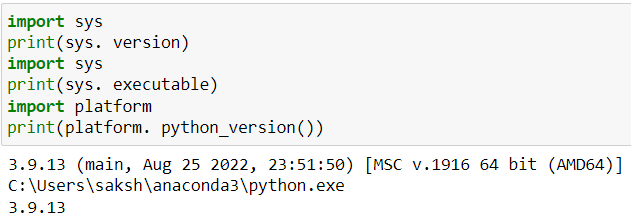
\includegraphics[width=0.8\linewidth]{ScreenShort/Python_env.png}
    \caption{Python environment installation}
\end{figure}

\begin{figure}[h!]
    \centering
    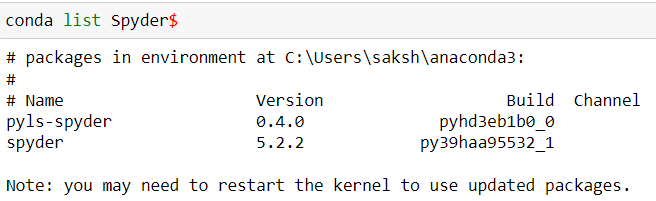
\includegraphics[width=0.8\linewidth]{ScreenShort/SpyderIDE.png}
    \caption{Spyder IDE}
\end{figure}

\begin{figure}[h!]
    \centering
    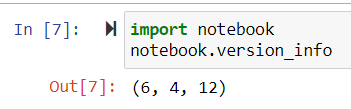
\includegraphics[width=0.8\linewidth]{ScreenShort/JPNotebook.png}
    \caption{Jupyter Notebook}
\end{figure}


\begin{figure}[h!]
    \centering
    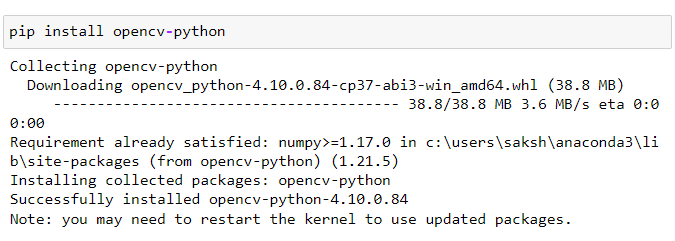
\includegraphics[width=0.8\linewidth]{ScreenShort/opencv.png}
    \caption{Command used to install OpenCV}
\end{figure}

\section{Task 3}
\textit{Generate / download a dataset of bird images!}\\
    In this assignment I selected three birds images: Cardinal, Sparrow and 
Red-Bellied Woodpecker. Fig. 5 is a color image of Cardinal, Fig. 6 is a color image of Sparrow and Fig. 7 is color image of Red-Bellied Woodpecker.


\begin{figure}[h!]
    \centering
    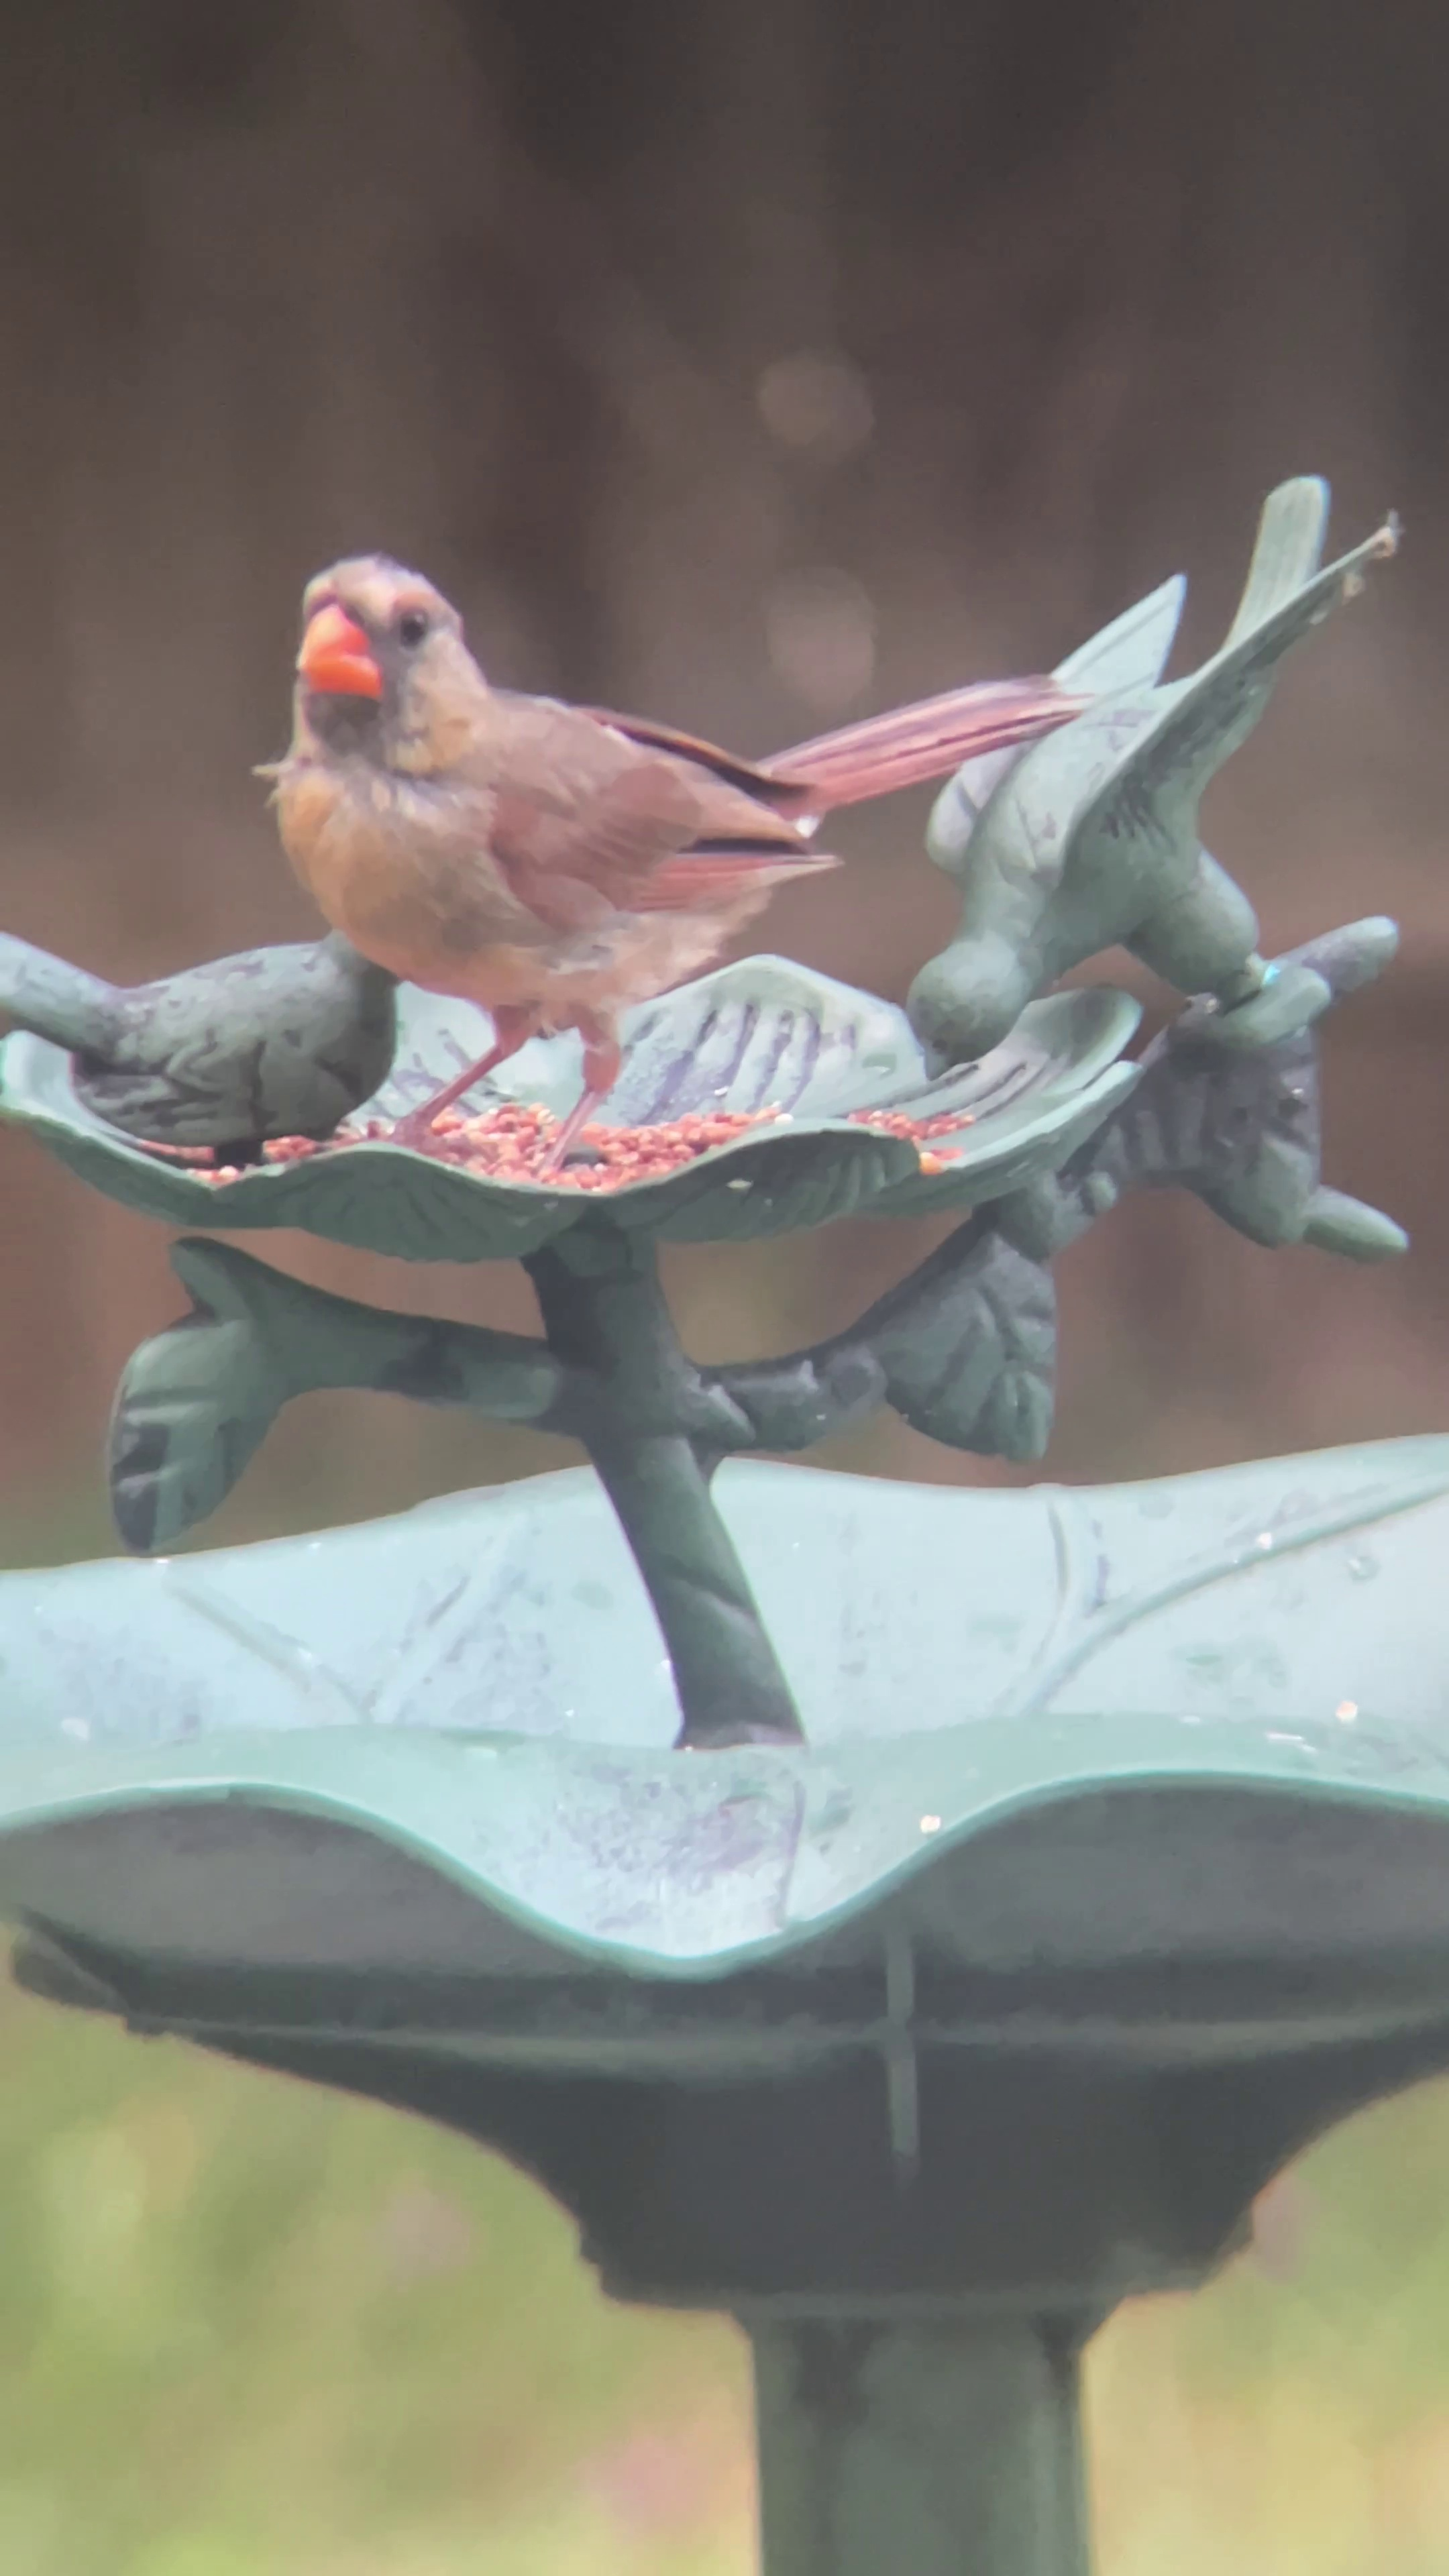
\includegraphics[width=0.6\linewidth, height=5cm]{ScreenShort/Cardinal.jpg}
    \caption{Cardinal (image0)}
\end{figure}

\begin{figure}[h!]
    \centering
    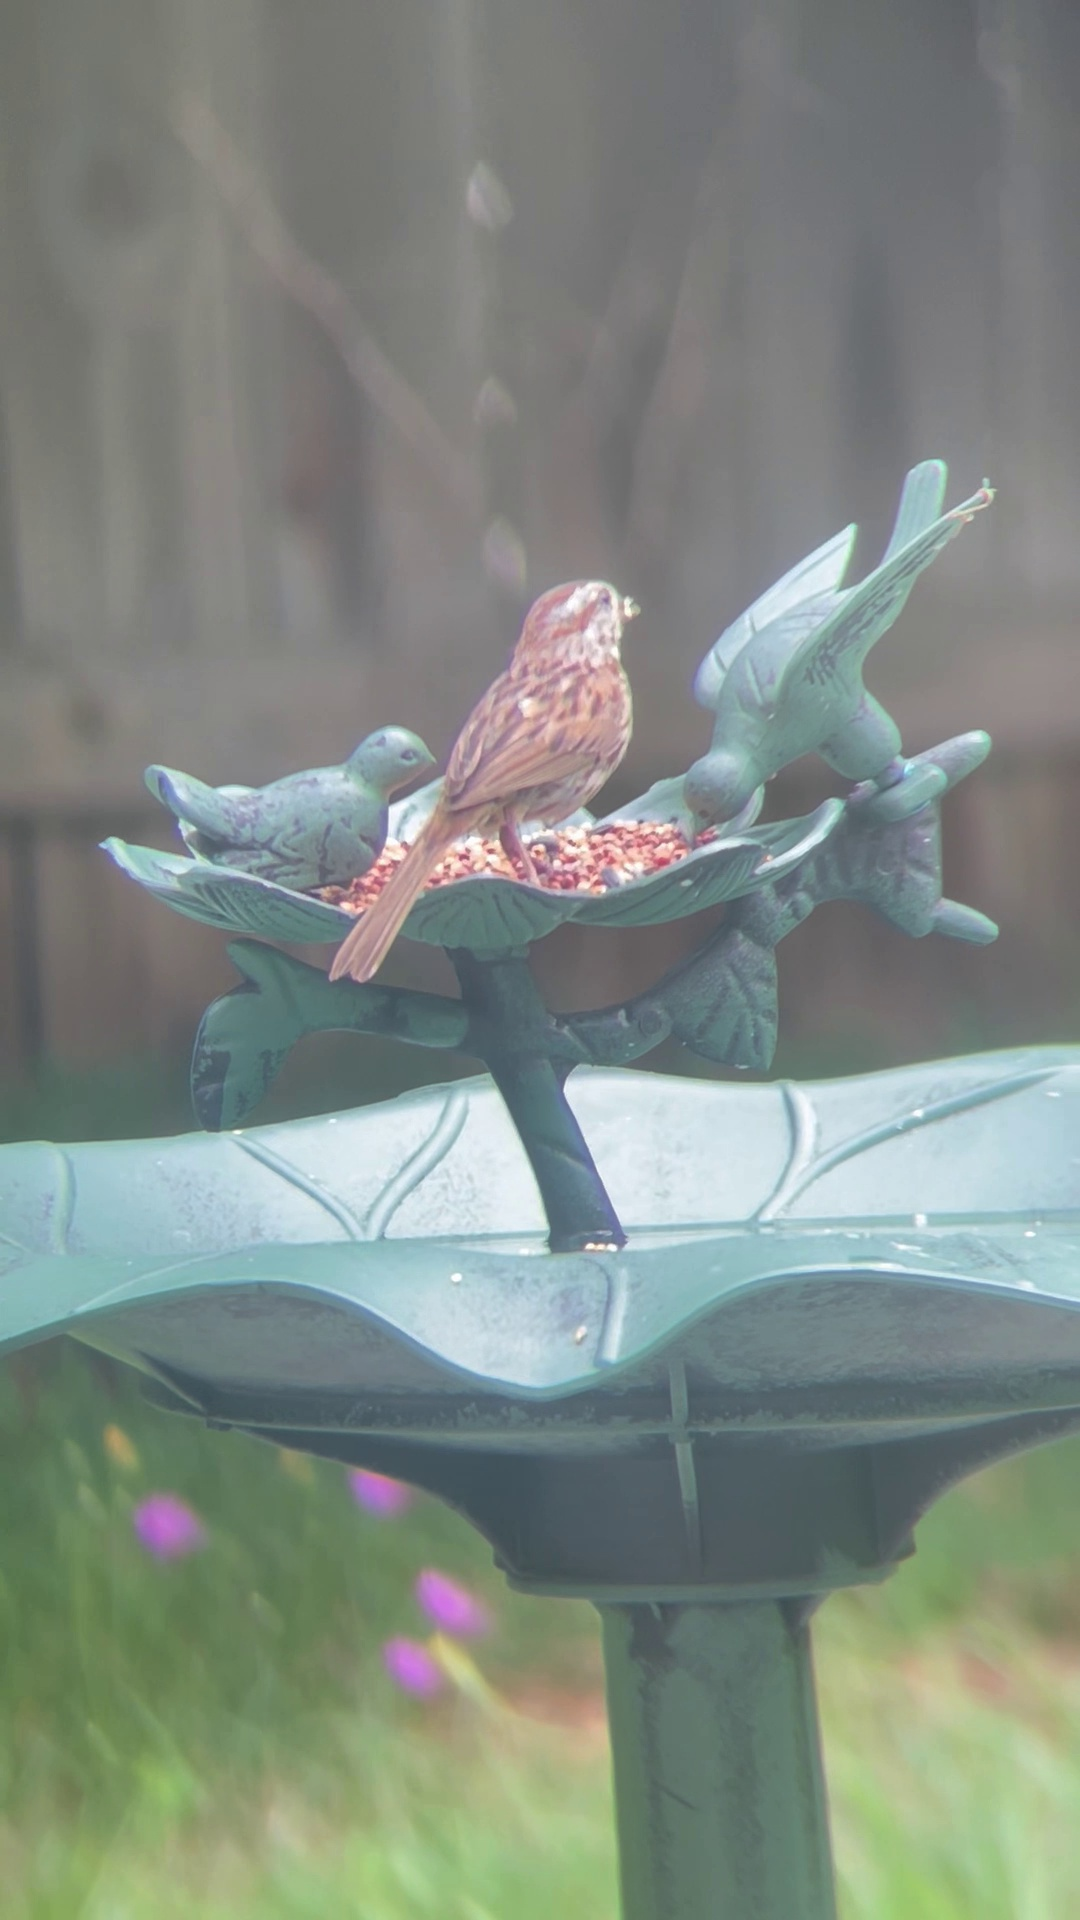
\includegraphics[width=0.6\linewidth, height=5cm]{ScreenShort/Sparrow.jpg}
    \caption{Sparrow (image1)}
\end{figure}

\begin{figure}[h!]
    \centering
    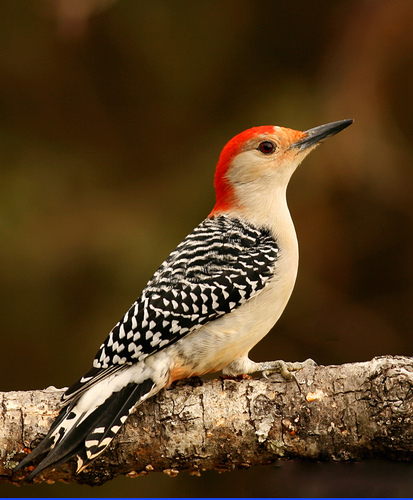
\includegraphics[width=0.6\linewidth, height=5cm]{ScreenShort/Red Bellied Woodpecker.jpg}
    \caption{Red-Bellied Woodpecker (image2)}
\end{figure}

\section{Task 4}
\textit{Write a simple code to read your selected images and display them on the programming environment!}\\
Before we start with programming first we need to import some library such as pandas, matplotlib, numpy, cv2. In this task we need to read these three color images and display it in RGB channel images. After that we converted that image into grayscale and display the dimensions of all this three images.
\begin{figure}[h!]
    \centering
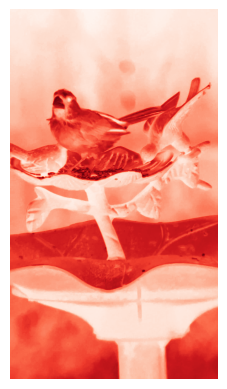
\includegraphics[width=0.3\linewidth, height=2.5cm]{ScreenShort/R_image0.png}
    \caption{Red\_image0}
\end{figure}
\begin{figure}[h!]
    \centering
    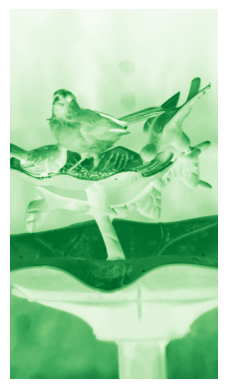
\includegraphics[width=0.3\linewidth, height=2.5cm]{ScreenShort/G_image0.png}
    \caption{Green\_image0}
\end{figure}
\begin{figure}[h!]
    \centering
    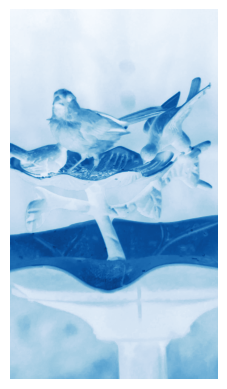
\includegraphics[width=0.3\linewidth, height=2.5cm]{ScreenShort/B_image0.png}
    \caption{Blue\_image0}
\end{figure}

\begin{figure}[h!]
    \centering
    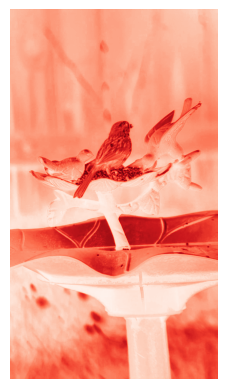
\includegraphics[width=0.3\linewidth, height=2.5cm]{ScreenShort/R_image1.png}
    \caption{Red\_image1}
\end{figure}
\begin{figure}[h!]
    \centering
    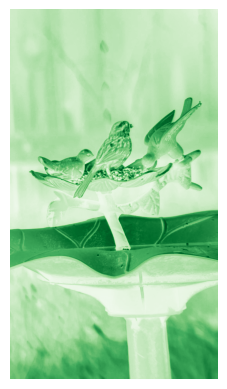
\includegraphics[width=0.3\linewidth, height=2.5cm]{ScreenShort/G_image1.png}
    \caption{Green\_image1}
\end{figure}
\begin{figure}[h!]
    \centering
    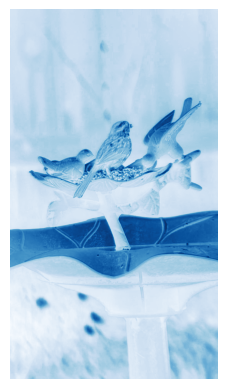
\includegraphics[width=0.3\linewidth, height=2.5cm]{ScreenShort/B_image1.png}
    \caption{Blue\_image1}
\end{figure}

\begin{figure}[h!]
    \centering
    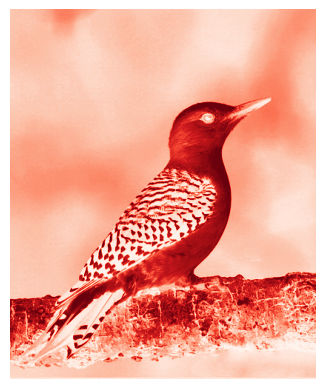
\includegraphics[width=0.3\linewidth, height=2.5cm]{ScreenShort/R_image2.png}
    \caption{Red\_image2}
\end{figure}
\begin{figure}[h!]
    \centering
    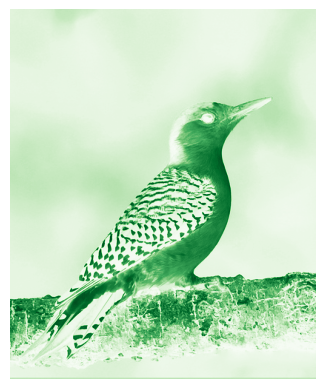
\includegraphics[width=0.3\linewidth, height=2.5cm]{ScreenShort/G_image2.png}
    \caption{Green\_image2}
\end{figure}
\begin{figure}[h!]
    \centering
    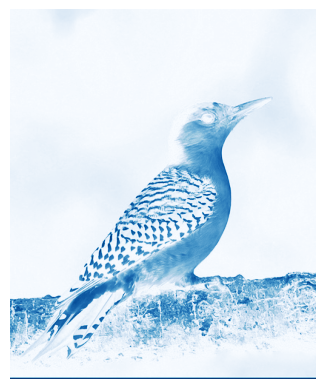
\includegraphics[width=0.3\linewidth, height=2.5cm]{ScreenShort/B_image2.png}
    \caption{Blue\_image2}
\end{figure}

\begin{figure}[h!]
    \centering
    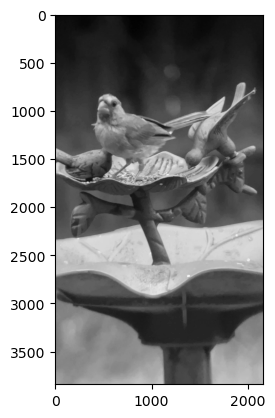
\includegraphics[width=0.6\linewidth, height=6cm]{ScreenShort/gray_image0.png}
    \caption{Grayscale\_image0}
\end{figure}

\begin{figure}[h!]
    \centering
    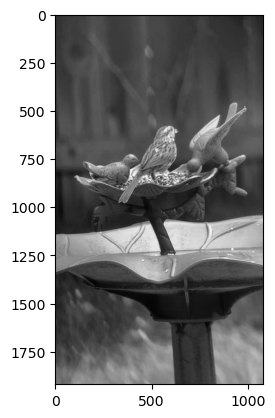
\includegraphics[width=0.6\linewidth, height=6cm]{ScreenShort/gray_image1.png}
    \caption{Grayscale\_image1}
\end{figure}

\begin{figure}[h!]
    \centering
    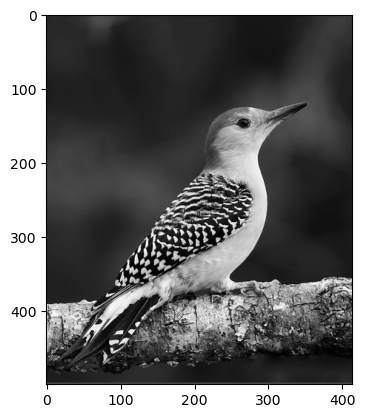
\includegraphics[width=0.6\linewidth, height=5cm]{ScreenShort/gray_image2.png}
    \caption{Grayscale\_image2}
\end{figure}
\newpage
\section{Task 5}
\textit{Resize the images to reduce their dimensions!}\\
  In this task, we need to resize the grayscale images such that the output dimensions are divisible by 16, while preserving their original aspect ratios as closely as possible.

The aspect ratio is the relationship between an image's width and height. It has been specified that the grayscale images must be resized to a height of 256 pixels, and the aspect ratio should be maintained when calculating the width of the target resized image. The new width of the resized image is calculated using the following formula:

\begin{equation}
    \text{aspect\_ratio} = \frac{\text{original\_w}}{\text{original\_h}}
\end{equation}

\begin{equation}
    \text{new\_width} = \text{target\_height} \times \text{aspect\_ratio}
\end{equation}

Where:\\
- \(\text{original\_w}\) is the original width of the image,\\
- \(\text{original\_h}\) is the original height of the image,\\
- \(\text{target\_height}\) is the desired height for the resized image,\\
- \(\text{aspect\_ratio}\) is the ratio of the width to the height of the image,\\
- \(\text{new\_width}\) is the calculated width that maintains the original aspect ratio of the image.\\

After calculating the new width of the images, we need to ensure that the new height and width of each image are divisible by 16. Therefore, the resulting resized image dimensions are as follows:\\
image0: (256, 144)\\
image1: (256, 144)\\
image2: (256, 208)\\

\section{Task 6}
\textit{Generate block-feature vectors!}\\
In this task, I first created blocks of 16x16 pixels from the image. In Fig. 20, we can see an example of one such 16x16 pixel block. Next, I flattened the block into a 1D vector of size 16x16 = 256. After creating the feature vector, which has a size of 256, I appended labels to each feature vector with values 0, 1, and 2. The label for image0 is 0, for image1 it is 1, and for image2 it is 2.

After generating the feature vectors for each image—where each row represents a feature vector. I combined all the feature vectors into one dataframe. Finally, I generated a spreadsheet named feature\_vectors.csv, which stores the feature vectors for all the images (image0, image1, and image2).
\begin{figure}[h!]
    \centering
    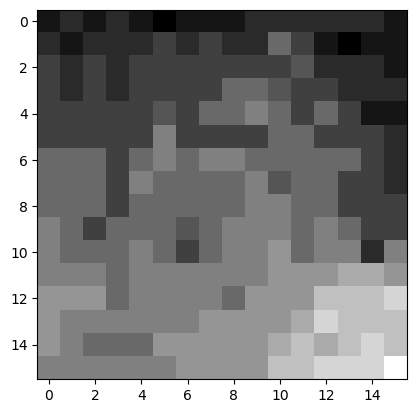
\includegraphics[width=0.6\linewidth, height=5cm]{ScreenShort/block16x16.png}
    \caption{Block of 16x16 pixels}
\end{figure}

\section{Task 7}
\textit{Generate sliding block-feature vectors!}\\
This task is about to create new feature vector with the idea of sliding block. The idea behind it is move a block of fixed size (in this case 16x16 pixels) across an image, extracting and flattening each block into 1D feature vector. The function slides the window across the image using a step size, which determines the overlap between consecutive blocks. \\
Block size: Defines the dimensions of the window (16x16 pixels in this case).\\
Step size: Controls how much the window moves with each step (8 pixels in this case).\\
Flattening: The block is flattened into a 1D array of size 256 (16x16).\\
The sliding window block plays a crucial role in breaking down images into smaller block with overlap between consecutive blocks, allowing for effective feature extraction that captures local information. It is useful in tasks such as image classification or object detection.\\
After creating sliding window feature vectors for each images with the labels I combined all the feature vectors into one dataframe. Finally, I generated a spreadsheet named sliding\_window\_feature\_vectors.csv, which stores the  sliding window feature vectors for all the images (image0, image1, and image2). Fig. 21 and Fig. 22 illustrate the concept of generating block feature vectors and sliding block feature vectors.
\begin{figure}[h!]
    \centering
    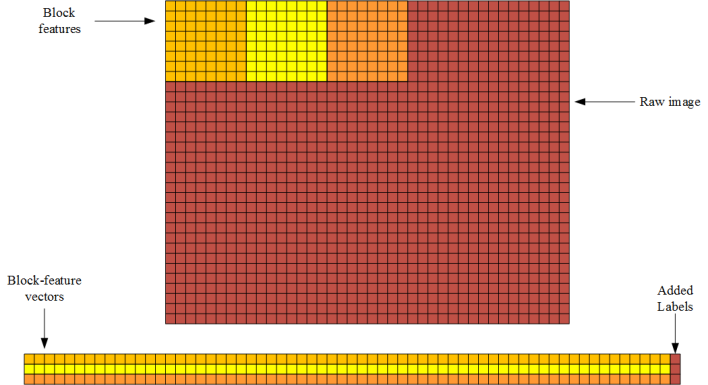
\includegraphics[width=0.6\linewidth, height=5cm]{ScreenShort/BFV.png}
    \caption{Generating block feature vectors}
\end{figure}
\begin{figure}[h!]
    \centering
    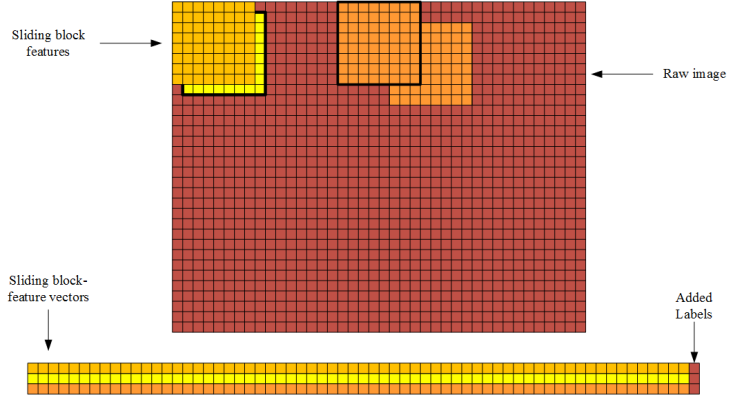
\includegraphics[width=0.6\linewidth, height=5cm]{ScreenShort/SBFV.png}
    \caption{Generating sliding block feature vectors}
\end{figure}

\section{Task 8}
\textit{Derive statistical descriptors!}\\
In this task we need to extract some  statistical information (e.g., number of observations, dimension of the data, mean of each feature, etc.) from datasets.Table 1 show the statistical values for image0, image1 and image2.\\
Also presented the visual representation of image0, image1 and image2 in histogram and scatter plot.

\begin{table}[h!]
\centering
\caption{Statistical Overview of Image 0, Image 1, and Image 2}
\begin{tabular}{|p{2cm}|c|c|c|}
\hline
\textbf{Statistic} & \textbf{Image 0} & \textbf{Image 1} & \textbf{Image 2} \\
\hline
\textbf{Number of observations} & 36,864 & 36,864 & 53,248 \\
\textbf{Dimension} & (256, 144) & (256, 144) & (256, 208) \\
\textbf{Min} & 52 & 74 & 0 \\
\textbf{Max} & 246 & 254 & 255 \\
\textbf{Mean} & 126.809 & 134.703 & 65.974 \\
\textbf{Std Dev} & 49.264 & 34.377 & 55.733 \\
\hline
\end{tabular}
\label{tab:statistics}
\end{table}

\begin{figure}[h!]
    \centering
    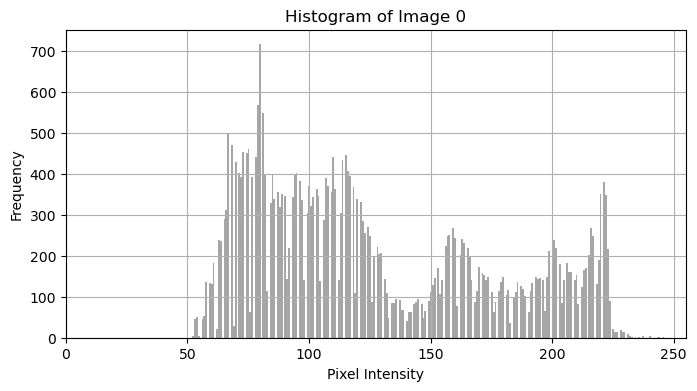
\includegraphics[width=0.6\linewidth, height=5cm]{ScreenShort/hist_image0.png}
    \caption{Histogram of Image0}
\end{figure}
\begin{figure}[h!]
    \centering
    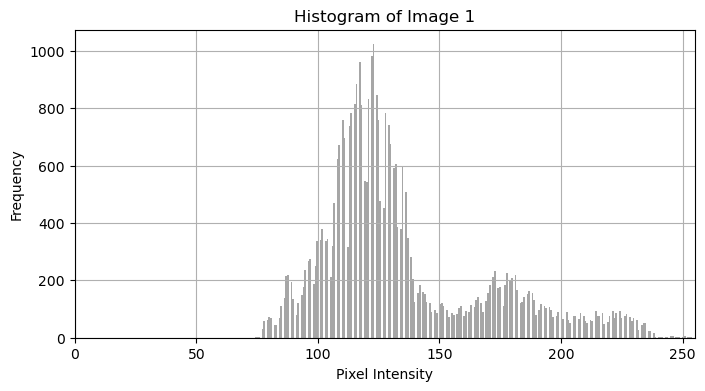
\includegraphics[width=0.6\linewidth, height=5cm]{ScreenShort/hist_image1.png}
    \caption{Histogram of Image1}
\end{figure}
\begin{figure}[h!]
    \centering
    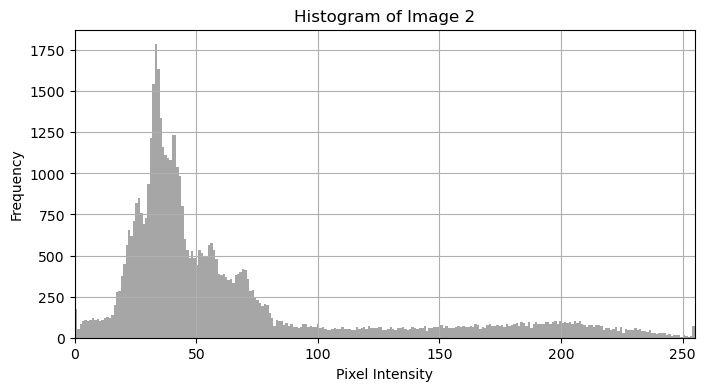
\includegraphics[width=0.6\linewidth, height=5cm]{ScreenShort/hist_image2.png}
    \caption{Histogram of Image2}
\end{figure}
\begin{figure}[h!]
    \centering
    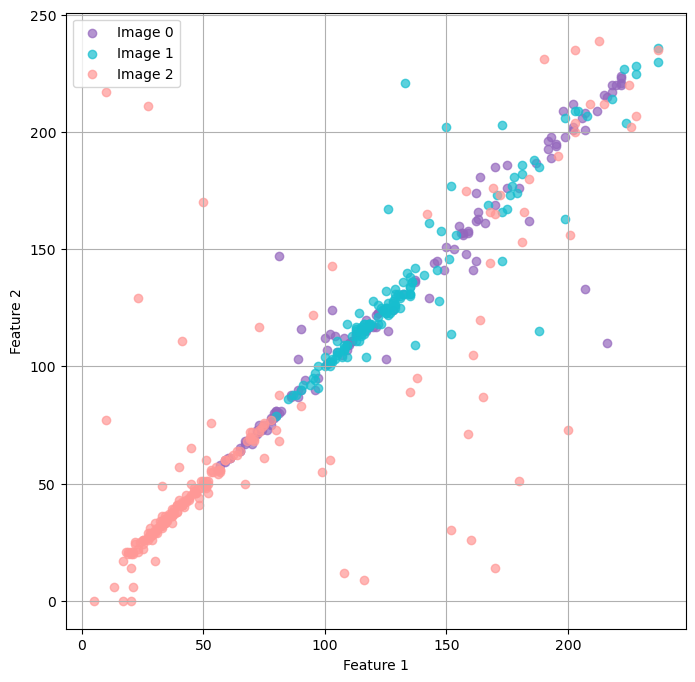
\includegraphics[width=0.6\linewidth, height=5cm]{ScreenShort/scat_image012.png}
    \caption{Scatter plot of image0, image1 and image2}
\end{figure}
\textbf{Is the dataset imbalanced, inaccurate, or incomplete?}\\

Imbalanced Data:Imbalanced data means the classes are not balanced. That means one or more classes have significantly fewer or more instances than the others.

I did the code for calculating class distribution and I get the below class distribution for label 0,1 and 2.\\
Class 0 : 144\\
Class 1 : 144\\
Class 2 : 208\\
Class 0 and Class 1 have the same number of instances (144 each). Class 2 has 208 instances, which is 64 more than Class 0 and Class 1. It could be considered slightly imbalanced because there is some variation. The ratio of the largest to smallest class is about 1.44 : 1. This level of imbalance is relatively mild and may not cause significant problems for many machine learning algorithms
\begin{figure}[h!]
    \centering
    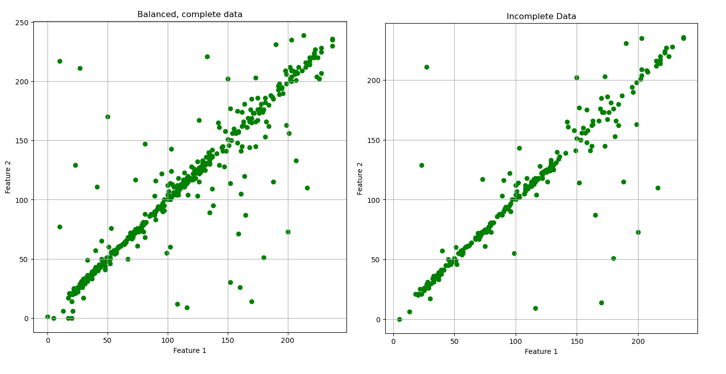
\includegraphics[width=0.9\linewidth, height=5cm]{ScreenShort/incomplete.png}
    \caption{Incomplete data}
\end{figure}

Inaccurate Data: Inaccurate data means the observation are not correct. It means some of the observations are not correctly labeled.
\begin{figure}[h!]
    \centering
    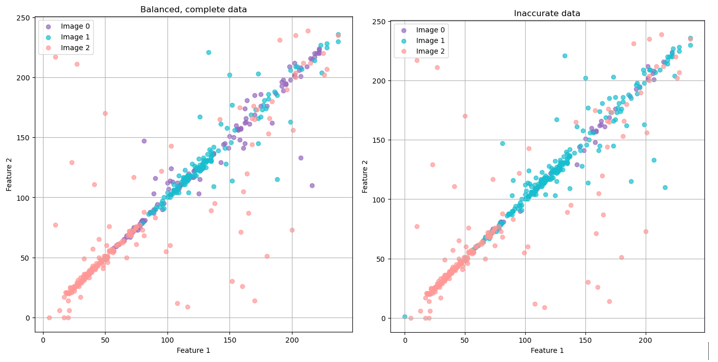
\includegraphics[width=0.9\linewidth, height=5cm]{ScreenShort/inaccurate.png}
    \caption{Inaccurate data}
\end{figure}

\textbf{Is it a trivial data or possibly a big data?}

If the data has complex structure(mixture Gaussian Model), classification of image is difficult and patterns are hidden in the plot then that data is called big data.

Above is the 2D ploting of feature 1 and 2 of image0,image1 and image2. Which show that it's very difficult to find the patterns in this plot. So we can say that it's big data. However, we can find some hidden patterns using standardization, normalization, linear transformation, and orthogonalization over the feature variables.

\textbf{Are they high dimensional?}

If n < p, then the data set is said to be high dimensional where n is number of observations and p is number of features. Accoding to this Image0, Image1 and Image2 all are not high dimensions.

\textbf{Do you need to standardize?}\\
Standardization is the process of transforming features to have a mean of 0 and a standard deviation of 1. It centers the data around zero and scales it to have unit variance. After calculating mean and standard deviation, the standardized means for image0, image1, and image2 are very close to zero, as approximately 0.
This indicates that the average pixel value across each of the images has been shifted to the center of the distribution.
\textbf{Do you need to standardize?}\\
Normalization scales the data between 0 and 1 or another range. It ensures that all features have a similar influence on the model, regardless of their original scales.
Normalization would involve scaling image0, image1 and image2 to a common range, such as [0, 1]. This ensures that both features contribute equally to the model, regardless of their original magnitudes.
Normalization prevents features with larger scales from dominating the model's training process and biases. It ensures that all features are treated equally and prevents numerical instabilities during optimization. Normalized features lead to more stable and efficient learning algorithms.

\section{Task 9}
\textit{Construct a feature space!}\\
In this task, I first created spreadsheets for each image, containing their individual feature vectors, named: image0.csv, image1.csv, and image2.csv. Following the task requirements, I then created a feature space by merging the feature vectors of image0 and image1, and named it image01.csv, with a dimension of (288, 257), where the 257th column contains the label. Similarly, I merged the feature vectors of image0, image1, and image2 to create a feature space for all three images, named image012.csv, with a dimension of (496, 257).

For the third sub-task, I randomized the placement of the feature vectors in both image01.csv and image012.csv and renamed them as random\_merged\_image01.csv and random\_merged\_image012.csv, respectively. The purpose of this randomization is to prepare the data for training a machine learning model.

\section{Task 10}
\textit{Display subspace!}\\
In this task we need to select the feature and plot the two-dimensional and three-dimensional. Fig. 29 show the two dimensional feature space for first and second feature and Fig. 30 show the three dimensional feature space for first, second and third feature. 
\begin{figure}[h!]
    \centering
    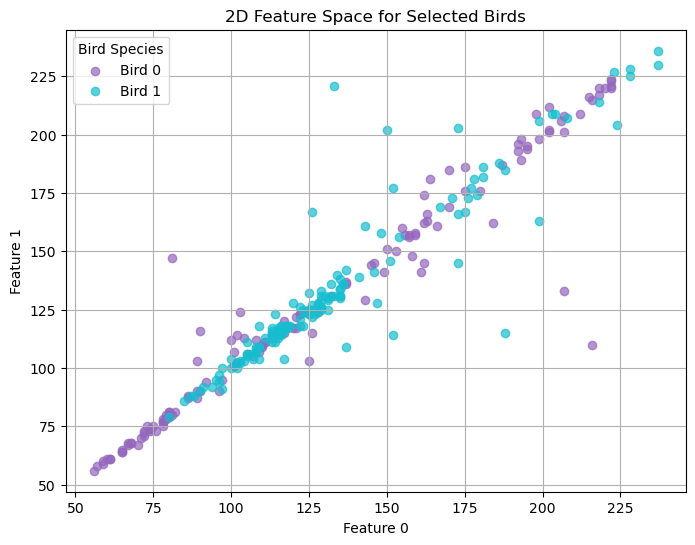
\includegraphics[width=0.9\linewidth, height=5cm]{ScreenShort/2D_image01.png}
    \caption{2D Feature Space}
\end{figure}

\begin{figure}[h!]
    \centering
    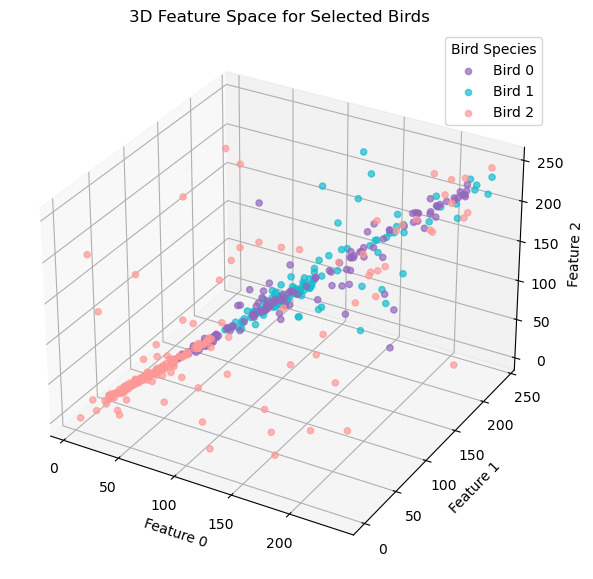
\includegraphics[width=0.9\linewidth, height=7cm]{ScreenShort/3D_image012.png}
    \caption{3D Feature Space}
\end{figure}

2D Feature Space: The 2D scatter plot shows a significant overlap between the two bird species (Bird 0 and Bird 1) based on the chosen features (Feature 0 and Feature 1). This overlap indicates that the selected features alone may not be enough to distinguish between the two bird species effectively.
The scatter points seem to align along a diagonal axis, suggesting that there is some correlation between Feature 0 and Feature 1. Both bird species follow a similar linear pattern, further complicating classification based on these two features alone.
The plot shows that in some regions, especially in the central portion of the scatter plot, it would be difficult to classify the bird species based on these features due to high overlap.

3D Feature Space: Introducing a third feature (Feature 2) slightly improves the separation of the bird species. While Bird 0 and Bird 1 still overlap, there is better visual differentiation compared to the 2D plot. The inclusion of Bird 2 (the green points) adds a new class, which is more spread out and distinct.
In 3D space, you can observe that Bird 2 is more separable due to the variation in Feature 2, and its points are more dispersed compared to the other two bird species. The added dimension helps in visualizing a bit more variance among the species, especially for Bird 2.
Despite the third dimension, Bird 0 and Bird 1 still exhibit significant overlap, which indicates that additional or more discriminative features might be needed for clearer separation between these two classes.

\section{Task 11}
\textit{Make appropriate changes to your Python code such that it can read any number of images from a folder that consists of many similar images, generate a feature space/s, and a spreadsheet/s for the feature spaces!}\\
In this task, I modified my code to read all images from the folder and create the feature space for each of them and generated spreadsheet with name folder\_feature\_vectors.csv.

\section{Task 12}
\subsection{Impact of Block Size on Vector Count and Feature Space Dimensionality}
The choice of block size plays a key role in shaping the dimensionality of the feature space and the number of vectors that represent the data. When transforming raw data into a feature space, block size directly affects how the data is divided, influencing both the complexity and the performance of classifiers. This section explores how varying block sizes impact the feature space and the classifiers' functionality within it.

\subsection{ Dimensionality of the Feature Space}
The dimensionality of the generated feature space is highly dependent on the selected block size. Larger block sizes tend to capture more complex, detailed representations of the data, revealing finer patterns. However, this also results in higher dimensionality, which can cause problems such as increased computational demands and the "curse of dimensionality" (where too many dimensions complicate analysis).

Conversely, smaller block sizes produce simpler, lower-dimensional representations, which may be easier to compute but can miss important details in the data.

Choosing the right block size involves finding a balance between capturing enough detail for the task (such as classification or regression) and ensuring that the computational load remains manageable. The choice should be informed by the characteristics of the dataset and the specific goals of the analysis.

\subsection{Number of Vectors in the Feature Space}
The number of vectors that represent the data in the feature space is also influenced by block size. Larger blocks cover more area, resulting in fewer but broader vectors. This reduces the total number of vectors but may fail to capture finer variations in the data. Smaller blocks, on the other hand, increase the number of vectors, allowing for a more detailed representation of the data but potentially introducing noise or redundancy.

The number of vectors is important because it affects the classifier’s ability to interpret and process the data. Too few vectors may cause the classifier to miss subtle patterns, while too many vectors may lead to overfitting or inefficiencies due to noise.

\subsection{Impact on the Classifier}
The choice of block size has a significant impact on the classifier's performance. A classifier trained on a high-dimensional feature space (resulting from larger block sizes) may be more sensitive to changes in the data and can capture finer details, but it is also at higher risk of overfitting. In contrast, a classifier operating in a lower-dimensional feature space (from smaller block sizes) may be more stable but might overlook important nuances in the data.

Additionally, the block size affects more than just model complexity; it also influences computational efficiency and generalization ability. Selecting the optimal block size ensures that the classifier can balance accuracy and efficiency, aligning with the task's goals and the data's inherent characteristics.
\\[1em]
\maketitle{\textbf{Assignment 2: Feature Space to a Classifier}}


\section{Task 1}
\textit{Complete and extend the tasks of assignment 1}\\
In this assignment, we build on the work from Assignment 1 by using four specific categories of data frames that I generated previously. These data frames are: block feature vectors image01 and image012, as well as window block feature vectors sw\_image01 and sw\_image012. For clarity and consistency, I refer to these data frames as image01, image012, sw\_image01, and sw\_image012 in my code. To use these data frames in this assignment, I imported their CSV files and randomized the rows for future operations.

Once all datasets were imported, I split each one into an 80:20 ratio, where 80\% of the data was assigned to training and 20\% to testing. After dividing each of the four datasets, I saved these subsets with filenames appended by the suffixes \_train.csv for training data and \_test.csv for test data.

After completing these tasks, the next step is to select two features from each category of the training and testing sets and plot their histograms. I selected feature numbers 4 and 7 for all categories. Figures 31 to 34 display the resulting histogram plots. Table 2 show the mean and variance of features for training and testing datasets.


\begin{figure}[h!]
    \centering
    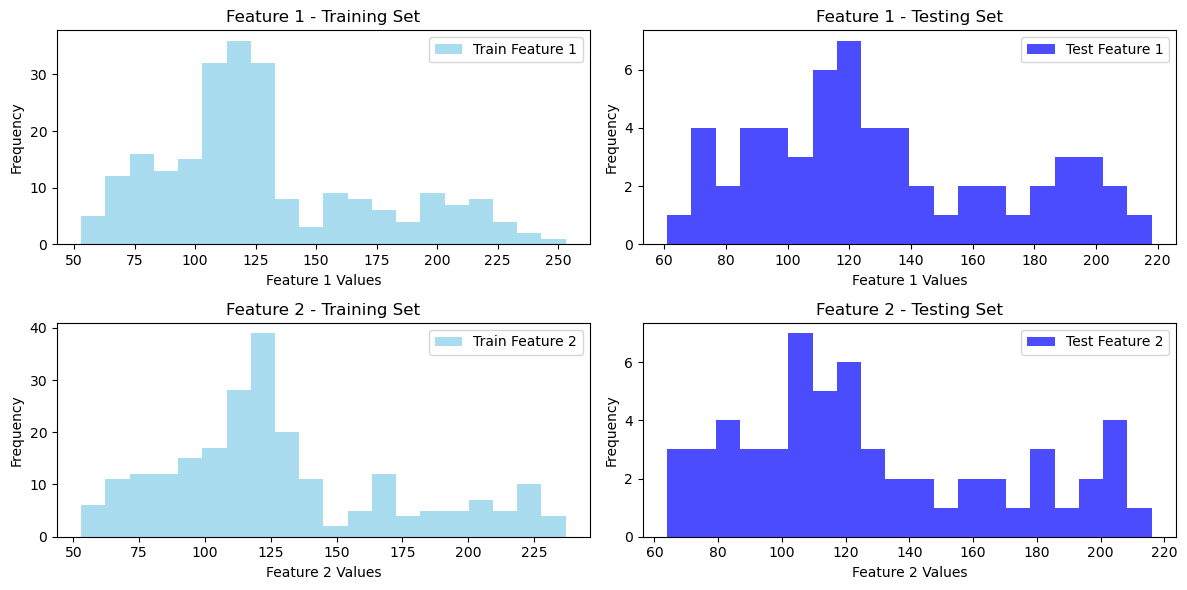
\includegraphics[width=1.0\linewidth]{ScreenShort/hist_image01_train_test.png}
    \caption{Histogram of image01\_train and image01\_test}
\end{figure}

\begin{figure}[h!]
    \centering
    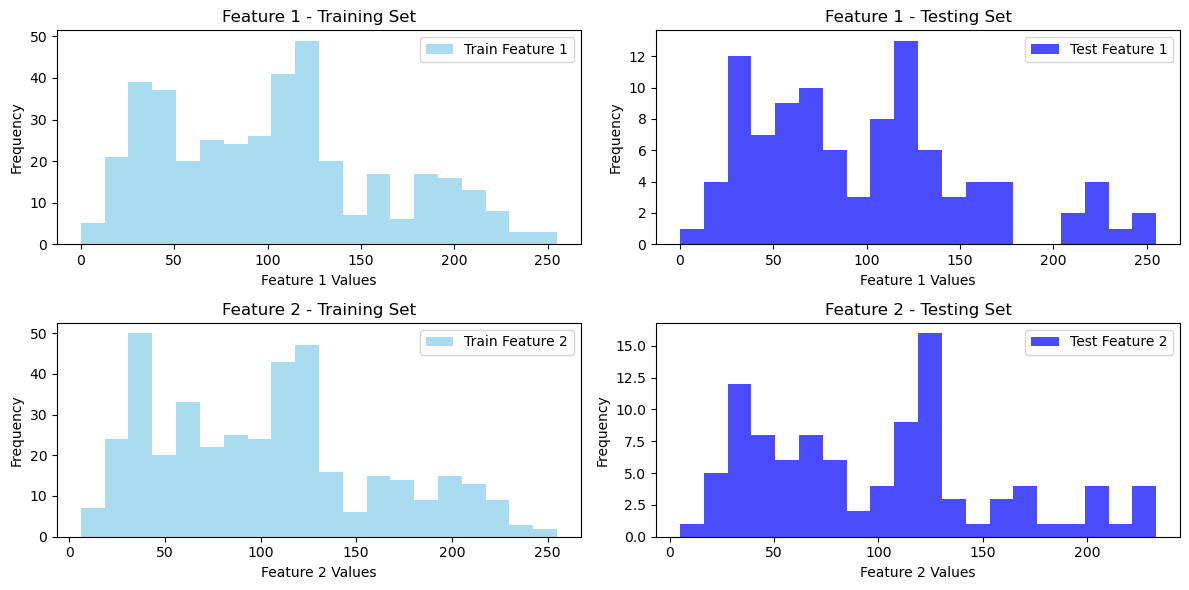
\includegraphics[width=1.0\linewidth]{ScreenShort/hist_image012_train_test.png}
    \caption{Histogram of image012\_train and image012\_test}
\end{figure}

\begin{figure}[h!]
    \centering
    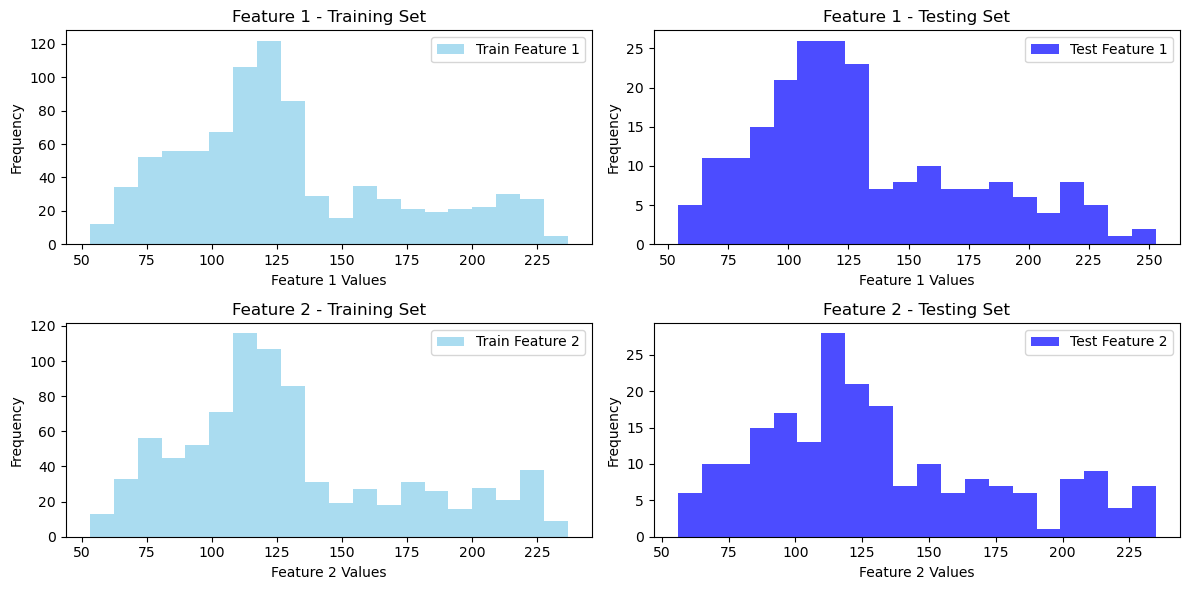
\includegraphics[width=1.0\linewidth]{ScreenShort/hist_sw_image01_train_test.png}
    \caption{Histogram of sw\_image01\_train and sw\_image01\_test}
\end{figure}

\begin{figure}[h!]
    \centering
    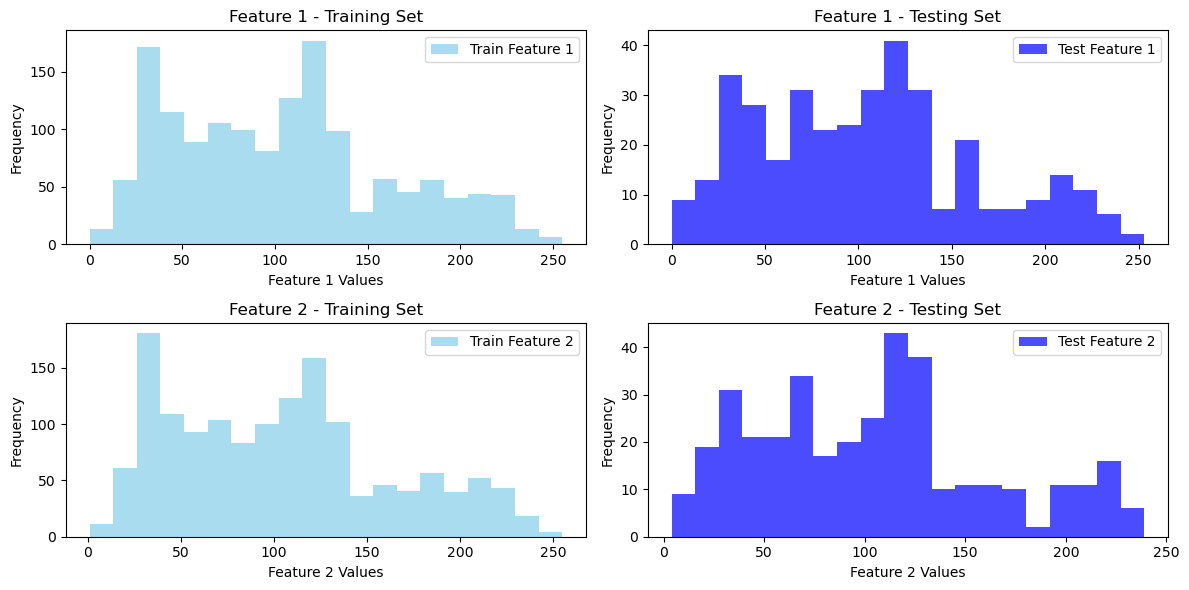
\includegraphics[width=1.0\linewidth]{ScreenShort/hist_sw_image012_train_test.png}
    \caption{Histogram of sw\_image012\_train and sw\_image012\_test}
\end{figure}


\begin{table}[h!]
\centering
\scriptsize % Reduces font size to fit within two-column format
\caption{Mean and Variance of Features for Training and Testing Datasets}
\begin{tabular}{|p{2.9cm}|c|c|c|c|c|}
\hline
\textbf{} & \multicolumn{2}{c|}{\textbf{Feature 1}} & \multicolumn{2}{c|}{\textbf{Feature 2}} \\ \hline
\textbf{Dataset} & \textbf{Mean} & \textbf{Variance} & \textbf{Mean} & \textbf{Variance} \\ \hline
image01\_train & 127.8 & 1931.6 & 128.8 & 1952.3 \\ \hline
image01\_test & 130.0 & 1649.1 & 128.5 & 1747.9 \\ \hline
image012\_train & 102.6 & 3421.5 & 103.1 & 3351.7\\ \hline
image012\_test & 100.0 & 3400.9 & 99.6 & 3228.5 \\ \hline
sw\_image01\_train & 128.1 & 1777.8 & 129.9 & 1914.9 \\ \hline
sw\_image01\_test & 130.3 & 2026.8 & 131.1 & 2034.5 \\ \hline
sw\_image012\_train & 103.1 & 3345.1 & 103.8 & 3435.1 \\ \hline
sw\_image012\_test & 104.3 & 3424.2 & 103.6 & 3368.5 \\ \hline
\end{tabular}
\end{table}

Using the same two features, we generated scatter plots for each category of the training and testing datasets. Figures 35 through 42 display these scatter plots.

\begin{figure}[h!]
    \centering
    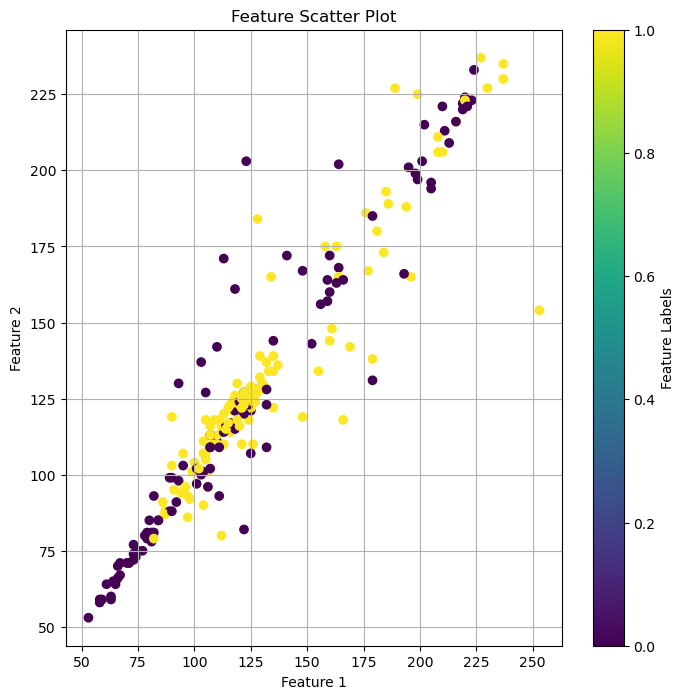
\includegraphics[width=1.0\linewidth, height=7cm]{ScreenShort/scat_image01_train.png}
    \caption{Scatter plot of image01\_train}
\end{figure}

\begin{figure}[h!]
    \centering
    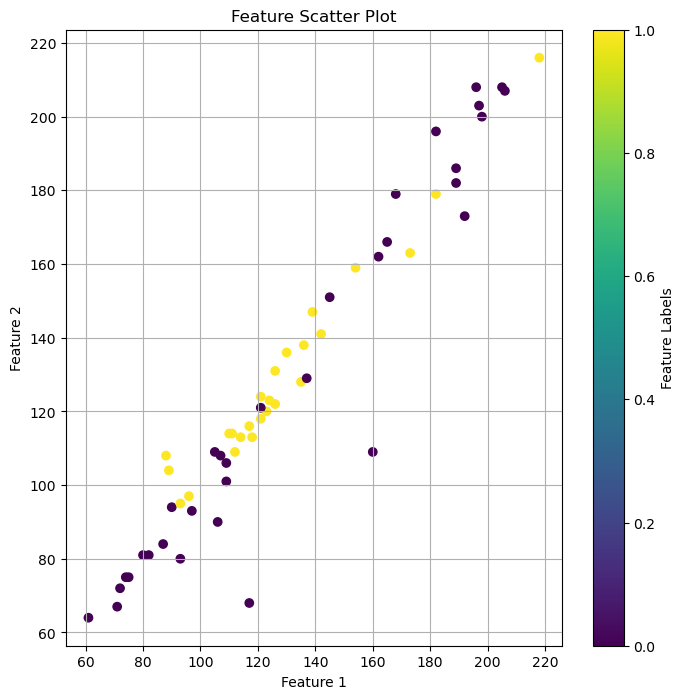
\includegraphics[width=1.0\linewidth, height=7cm]{ScreenShort/scat_image01_test.png}
    \caption{Scatter plot of image01\_test}
\end{figure}

\begin{figure}[h!]
    \centering
    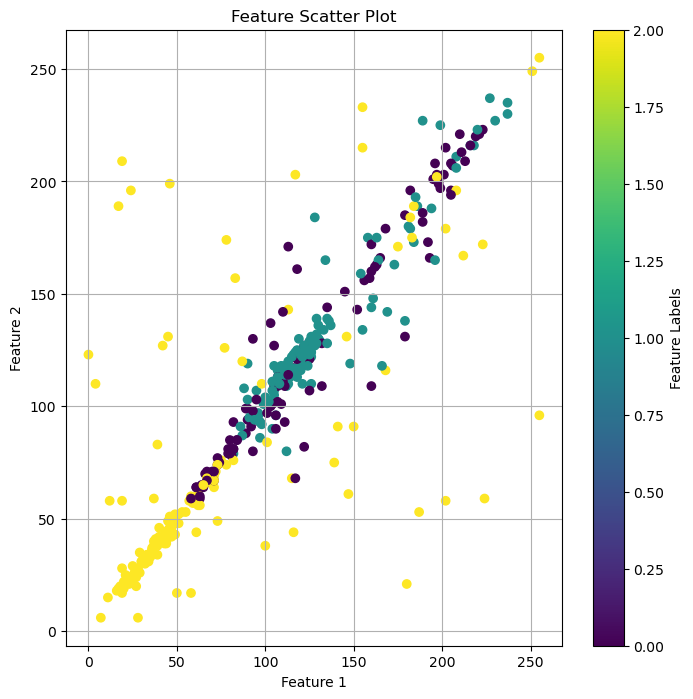
\includegraphics[width=1.0\linewidth, height=7cm]{ScreenShort/scat_image012_train.png}
    \caption{Scatter plot of image012\_train}
\end{figure}

\begin{figure}[h!]
    \centering
    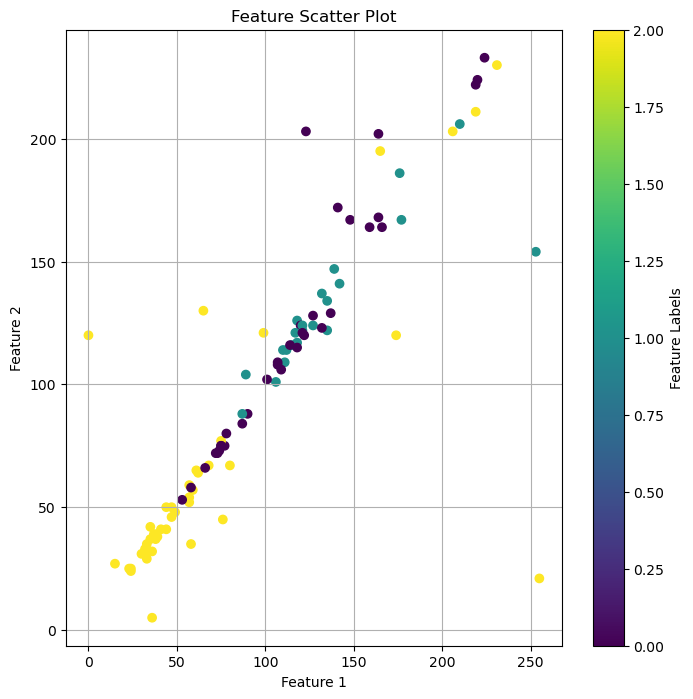
\includegraphics[width=1.0\linewidth, height=7cm]{ScreenShort/scat_image012_test.png}
    \caption{Scatter plot of image012\_test}
\end{figure}

\begin{figure}[h!]
    \centering
    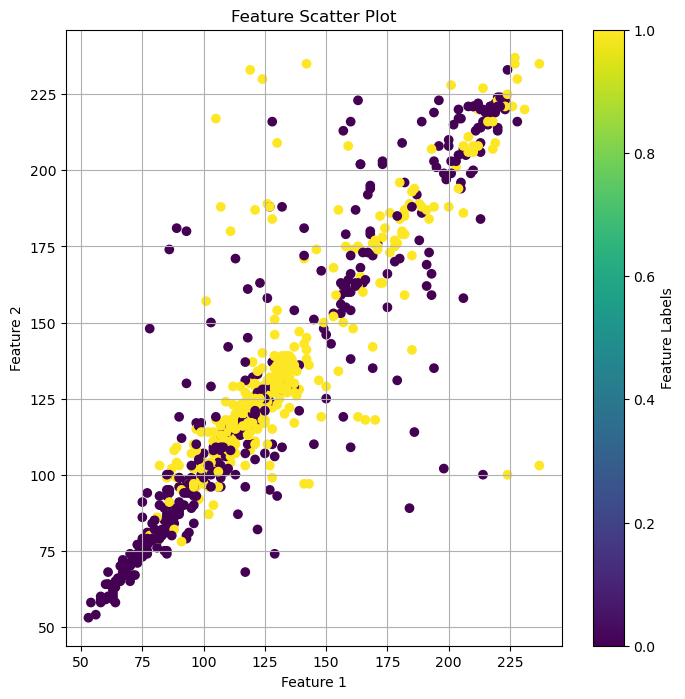
\includegraphics[width=1.0\linewidth, height=7cm]{ScreenShort/scat_sw_image01_train.png}
    \caption{Scatter plot of sw\_image01\_train}
\end{figure}

\begin{figure}[h!]
    \centering
    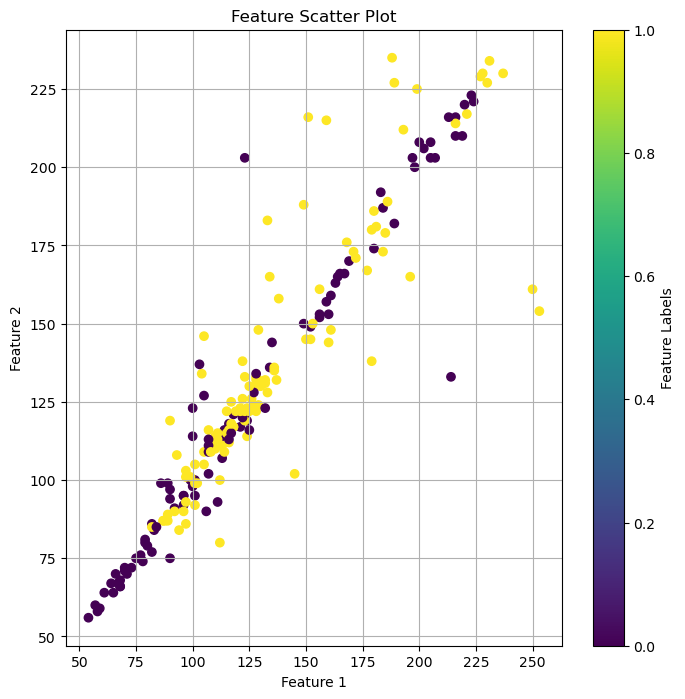
\includegraphics[width=1.0\linewidth, height=7cm]{ScreenShort/scat_sw_image01_test.png}
    \caption{Scatter plot of sw\_image01\_test}
\end{figure}

\begin{figure}[h!]
    \centering
    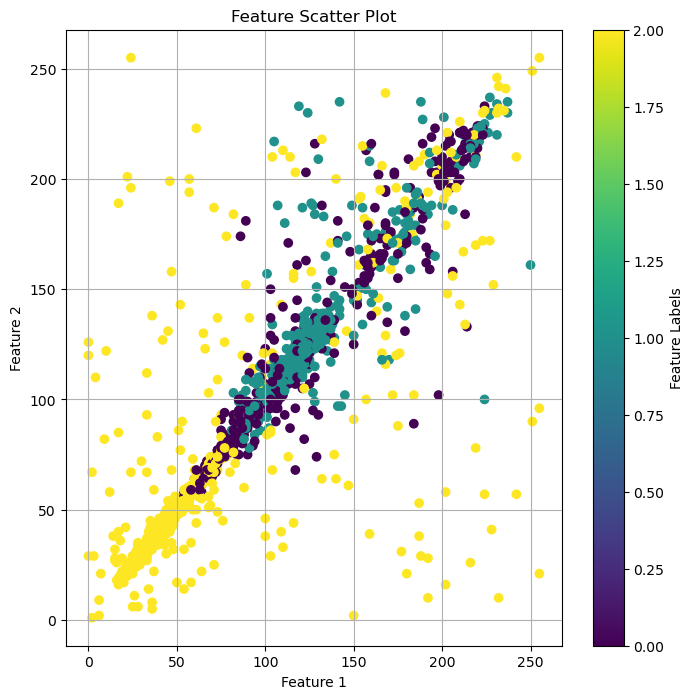
\includegraphics[width=1.0\linewidth, height=7cm]{ScreenShort/scat_sw_image012_train.png}
    \caption{Scatter plot of sw\_image012\_train}
\end{figure}

\begin{figure}[h!]
    \centering
    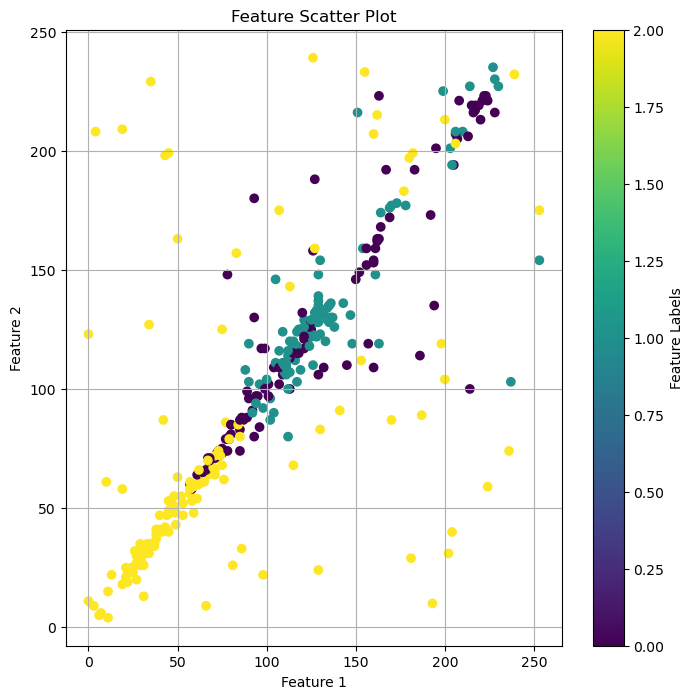
\includegraphics[width=1.0\linewidth, height=7cm]{ScreenShort/scat_sw_image012_test.png}
    \caption{Scatter plot of sw\_image012\_test}
\end{figure}

\section{Task 2}
\textit{Implementing a regression-based model}\\

In this task, we will implement a Lasso regression model using the training set for each data frame created in the previous task. To accomplish this, we will import the Lasso class from sklearn.linear\_model.

After generating the Lasso models for each feature vector category (image01, image012, sw\_image01, and sw\_image012), we will apply the trained models to the test sets of each dataset category. The predicted labels will then be added alongside the actual labels in the corresponding spreadsheets.

Finally, we will create a confusion matrix to compare the actual and predicted labels, allowing for evaluation of model performance across each feature vector category.

\begin{table}[h!]
\centering
\caption{Confusion matrix of lasso regression for image01}
\begin{tabular}{|c|c|}
\hline
16 & 17 \\ \hline
6  & 18 \\ \hline
\end{tabular}
\end{table}

\begin{table}[h!]
\centering
\caption{Confusion matrix of lasso regression for image012}
\begin{tabular}{|c|c|c|}
\hline
8 & 23 & 2 \\ \hline
6 & 15 & 1 \\ \hline
5 & 12 & 21 \\ \hline
\end{tabular}
\end{table}

\begin{table}[h!]
\centering
\caption{Confusion matrix of lasso regression for sw\_image01}
\begin{tabular}{|c|c|}
\hline
55 & 43 \\ \hline
55  & 58 \\ \hline
\end{tabular}
\end{table}

\begin{table}[h!]
\centering
\caption{Confusion matrix of lasso regression for sw\_image012}
\begin{tabular}{|c|c|c|}
\hline
31 & 77 & 1 \\ \hline
20 & 83 & 0 \\ \hline
16 & 40 & 92 \\ \hline
\end{tabular}
\end{table}

There are four different qualitative measures:
\\
1. accuracy\\
2. precision\\
3. sensitivity\\
4. specificity\\

I selected two qualitative measures accuracy and precision to quantify the performance of a machine learning model.

Accuracy: It describes the performance of the model based on the proportionality between the false positive and the true positive. If the accuracy is high, then it means that the classification of both classes are highly accurate (it is indicated by the double lines), and the false negative and false positives are ignorable.

Precision: It describes the performance of the model based on the proportionality between the false positives and the true positives. If the precision is high, then it means that the classification of A is precisely high (double line) with low false negatives

Below is the qualitative measures of lasso regression for each categories of datasets.
\\
image01:\\
Accuracy: 0.5964912280701754\\
Precision: 0.7272727272727273\\
\\
image012:\\
Accuracy: 0.4731182795698925\\
Precision: 0.5320175438596492\\
\\
sw\_image01:\\
Accuracy: 0.5355450236966824\\
Precision: 0.5\\
\\
sw\_image012:\\
Accuracy: 0.5722222222222222\\
Precision: 0.6223112929973788\\

\section{Task 3}
\textit{Implementing random forest or deep learning}\\
After importing RandomForestClassifier from sklearn.ensemble, I implemented the Random Forest model using the training sets of each feature vector category. Once the model was trained, I tested it on the test sets for all dataset categories and added the predicted labels alongside the actual labels in the corresponding spreadsheets, as previously done.

The next step was to create confusion matrices for the Random Forest model using the actual and predicted values, providing insight into the model's performance across the different categories.

\begin{table}[h!]
\centering
\caption{Confusion matrix of random forest for image01}
\begin{tabular}{|c|c|}
\hline
31 & 2 \\ \hline
3  & 22 \\ \hline
\end{tabular}
\end{table}

\begin{table}[h!]
\centering
\caption{Confusion matrix of random forest for image012}
\begin{tabular}{|c|c|c|}
\hline
24 & 8 & 2 \\ \hline
5 & 17 & 0 \\ \hline
6 & 0 & 37 \\ \hline
\end{tabular}
\end{table}

\begin{table}[h!]
\centering
\caption{Confusion matrix of random forest for sw\_image01}
\begin{tabular}{|c|c|}
\hline
80 & 17 \\ \hline
39 & 74 \\ \hline
\end{tabular}
\end{table}

\begin{table}[h!]
\centering
\caption{Confusion matrix of random forest for sw\_image012}
\begin{tabular}{|c|c|c|}
\hline
87 & 21 & 1 \\ \hline
21 & 82 & 0 \\ \hline
10 & 2 & 142 \\ \hline
\end{tabular}
\end{table}

Below is the qualitative measures of random forest for each categories of datasets.
\\
image01:\\
Accuracy: 0.9137931034482759\\
Precision: 0.911764705882353\\
\\
image012:\\
Accuracy: 0.7878787878787878\\
Precision: 0.7714774114774116\\
\\
sw\_image01:\\
Accuracy: 0.7333333333333333\\
Precision: 0.6722689075630252\\
\\
sw\_image012:\\
Accuracy: 0.8497267759562842\\
Precision: 0.8370825031841981\\

\section{Task 4}
\textit{Evaluation of the learning models}\\

After calculating accuracy and precision using confusion matrix we need to use built-in measures metrics.accuracy\_score and metrics.precision\_score from sklearn library to compare the performance of the models.

Below are the values of built-in  qualitative measures of Lasso regression for each categories of datasets.
\\
image01:\\
BuiltIn\_Accuracy: 0.5862068965517241\\
BuiltIn\_Precision: 0.6354679802955665\\
\\
image012:\\
BuiltIn\_Accuracy: 0.4444444444444444\\
BuiltIn\_Precision: 0.5913211057947899\\
\\
sw\_image01:\\
BuiltIn\_Accuracy: 0.5355450236966824\\
BuiltIn\_Precision: 0.5397681948289615\\
\\
sw\_image012:\\
BuiltIn\_Accuracy: 0.5628415300546448\\
BuiltIn\_Precision: 0.6708249230666691\\

Below are the values of built-in  qualitative measures of random forest for each categories of datasets.
\\
image01:\\
BuiltIn\_Accuracy: 0.9137931034482759\\
BuiltIn\_Precision: 0.9138776200135226\\
\\
image012:\\
BuiltIn\_Accuracy: 0.7878787878787878\\
BuiltIn\_Precision: 0.7986783586783587\\
\\
sw\_image01:\\
BuiltIn\_Accuracy: 0.7298578199052133\\
BuiltIn\_Precision: 0.7477367906696036\\
\\
sw\_image012:\\
BuiltIn\_Accuracy: 0.8497267759562842\\
BuiltIn\_Precision: 0.8571737129530962\\

\begin{table}[h!]
\centering
\scriptsize % Reduces font size to fit within two-column format
\caption{Difference between built-in measures values and confusion matrix based values for Lasso Regression}
\begin{tabular}{|p{2cm}|p{2cm}|p{2cm}|}
\hline
\textbf{Lasso Regression} & \textbf{Difference in Accuracy} & \textbf{Difference in Precision} \\ \hline
image01 & 0.01 & 0.091 \\ \hline
image012 & 0.028 & 0.059 \\ \hline
sw\_image01 & 0 & 0.039 \\ \hline
sw\_image012 & 0.009 & 0.048 \\ \hline
\end{tabular}
\label{table:lasso_regression}
\end{table} 

\begin{table}[h!]
\centering
\scriptsize % Reduces font size to fit within two-column format
\caption{Difference Between Built-in Measures Values and Confusion Matrix-Based Values for Lasso Regression}
\begin{tabular}{|p{2cm}|p{2cm}|p{2cm}|}
\hline
\textbf{Feature Vectors} & \textbf{Difference in Accuracy} & \textbf{Difference in Precision} \\ \hline
image01 & 0.31 & 0.002 \\ \hline
image012 & 0.0 & 0.02 \\ \hline
sw\_image01 & 0.003 & 0.07 \\ \hline
sw\_image012 & 0.0 & 0.02 \\ \hline
\end{tabular}
\label{table:lasso_regression}
\end{table}


After completing all tasks, we need to compare the results to determine which model and feature vector category combination is the most effective. The results are summarized in two tables: one for Lasso Regression and one for Random Forest, each displaying accuracy and precision values. By analyzing these tables, we can identify the superior model and feature vector category based on performance metrics.

\begin{table}[h!]
\centering
\caption{Lasso Regression Model Performance Using Built-in Measures}
\resizebox{\columnwidth}{!}{%
\begin{tabular}{|c|c|c|}
\hline
\textbf{Feature Vectors} & \textbf{Accuracy} & \textbf{Precision} \\
\hline
image01 & 0.586 & 0.635 \\
image012 & 0.444 & 0.591 \\
sw\_image01 & 0.535 & 0.539 \\
sw\_image012 & 0.562 & 0.670 \\
\hline
\end{tabular}%
}
\label{table:lasso_performance}
\end{table}

\begin{table}[h!]
\centering
\caption{Random Forest Model Performance Using Built-in Measures}
\resizebox{\columnwidth}{!}{%
\begin{tabular}{|c|c|c|}
\hline
\textbf{Feature Vectors} & \textbf{Accuracy} & \textbf{Precision} \\
\hline
image01 & 0.913 & 0.913 \\
image012 & 0.787 & 0.798 \\
sw\_image01 & 0.729 & 0.747 \\
sw\_image012 & 0.849 & 0.857 \\
\hline
\end{tabular}%
}
\label{table:random_forest_performance}
\end{table}

\textbf{Lasso Regression Model}: This model showing lower accuracy and precision scores across all feature vector categories. These scores suggest that the Lasso model might be struggling to fit the data as effectively as the Random Forest model.

\textbf{Random Forest Model}: Random Forest consistently outperforms Lasso in both accuracy and precision across all feature vector categories. The highest scores for both accuracy (0.913) and precision (0.913) occur with the image01 feature vector, indicating strong predictive power and reliable performance when using this feature set.

The \textbf{Random Forest model using the image01 feature vector} is the superior pairing among those evaluated. This feature set likely contains highly predictive information that Random Forest can leverage better than Lasso, which struggles with lower scores on this and other feature sets.


\end{document}
